\documentclass[12pt,a4paper]{report}
\usepackage[hmargin=3cm,vmargin=3cm]{geometry}
\usepackage{graphicx}
\usepackage{caption}
\usepackage{array}
\usepackage{listings}
\usepackage{hyperref}
\usepackage{float}
\usepackage{textcomp}
\usepackage{subcaption}
\newcommand\tab[1][0.5cm]{\hspace*{#1}}
\graphicspath{Images}

\hypersetup{
    colorlinks=true,
    linkcolor=black,
    urlcolor=blue
}
\begin{document}

\begin{figure}
\centering

\includegraphics[width = 0.3\textwidth]{iit}
\hspace{1cm}

\includegraphics[width = 0.4\textwidth]{fossee-logo}
\end{figure}

\title{\textbf{\textbf{Developing a Generic Purpose OpenModelica Library for Embedded Applications}}\vspace{5mm}\\
\vspace{5mm} \large Developer's Document - II\vspace{5mm} \\ \vspace{5mm}\small by\\  \vspace{1mm}  \large \textbf{Manas Ranjan Das}\\ \vspace{5mm} 
%\small Under the guidance of \\ \vspace{2mm}
%\large \textbf{Mentor: Mr. Manas Ranjan Das}\\ \vspace{3mm}
%\large \textbf{Prof. Kannan M. Moudgalya} \vspace{1mm}\\Department of Chemical Engineering  \vspace{1mm} \\IIT Bombay
}
%\vspace{1cm}

\maketitle

\tableofcontents
\listoffigures

\chapter{\textbf{Introduction}}
OpenModelica is a free and open source environment based on the Modelica modeling language for simulating, optimizing and analyzing complex dynamic systems. OpenModelica is used in academic and industrial environments. Industrial applications include the use of OpenModelica along with proprietary software in the fields of power plant optimization, automotive and water treatment. Models are either built through line by line code or graphical code in OpenModelica. OpenModelica can interact with C, Python languages and can call C, Python functions from within its models. OpenModelica is a powerful tool that can be used to design and simulate complete control systems. 

Our project was to implement model based design i.e. creating models for different embedded applications and generating C code that can be ported to the respective family of microcontrollers.We also worked towards Improving the Hardware In Loop (HIL) implementation on OpenModelica and microcontrollers like arduino and TivaC.The current implementation which is based on Inter Process Communication (IPC) needs to be made robust. Hence there is a need to come up with a less cumbersome  IPC for HIL.


\chapter{\textbf{Implementation}}
\section{Algorithm}
\begin{enumerate}
\item Once you have installed OpenModelica, launch OMEdit and open the OpenModelicaEmbedded package.
\item To use the above package you will also need to load Modelica\_DeviceDrivers package. The ‘synchronizeRealtime’ block present in this package is used to make the simulation of models real-time. All it does is that, it maps the time interval provided by you before simulation with clock your PC.
\item The components provided in this package are:
\begin{enumerate}
\item Pins: It contains Analog input, Analog output, Digital input, Digital output and Servo pins to perform corresponding function in model.
\item Boards: Any of the provided board can be used depending the one you are using, else use the ‘customBoard’ provided and vary it’s parameters to match the configuration of the development board you are using.
\end{enumerate}
\item Take a look at the examples provided along with the package to understand the basics structure of a model. Each model has ‘Board’ block which represents the development board used. This block when added to a model, on simulation calls a couple of functions present in ‘Internal > ExternalFunctions’ which set the initialisation parameters for communication like PORT, BAUD rate, etc.
\item These modelica functions present in ‘ExternalFunctions’ then call external C functions which perform the actual task the function is supposed to do.
\item These external C functions are bundled together and provided in the form of libraries. The Libraries used will be ‘*.dll’ in case of WindowsOS and ‘*.so’ in case of Linux.
\item After adding a board to your model add pins using blocks provided for the same. If you want to send some data from OpenModelica to connected microcontroller the use Analog/Digital Output Pin, and vice versa. Use Analog Pin while working with real data and Digital pin while working with Boolean.
\item These pin blocks again call functions in similar manner to either send or receive data.
\item Once your model is ready and check is successful, upload appropriate Firmware on microcontroller board connected.
\item The Firmware’s for Arduino and Tiva C borads have been provided along with the package. Open Arduino IDE if using Arduino board and Energia IDE if using Tiva C board and upload corresponding firmware on board.
\item The Firmware implements Firmata protocol to establish communication with OpenModelica.
\item Now go back to OpenModelica and simulate your model.
\end{enumerate}

\section{Making changes in source code}
\subsection{How to make changes to source code and make libraries}
{\textbf {Linux Operating System}}\\

Open the source codes by browsing to this location : OpenModelicaEmbedded \textrightarrow  Source.After making changes to the source code files open Terminal.Browse to OpenModelicaEmbedded \textrightarrow  Source folder using ‘cd’ command.Run command ‘make’ to generate shared object file('*.so').\\
\\
{\textbf {Windows Operating System}}\\

Open the source codes by browsing to this location : OpenModelicaEmbedded \textrightarrow  Source. After making changes to the source code, open Command Prompt (cmd).Browse to OpenModelicaEmbedded \textrightarrow  Source folder using ‘cd’ command.To compile the CPP files run the command: g++ -c modelPlugFirmata.cpp serial.cpp. To create a DLL from generated object files, run the command: g++ -shared -o modelPlugFirmata.dll modelPlugFirmata.o serial.o.Then copy the generated DLL file and paste it in folders: OpenModelicaEmbedded and Resources \textrightarrow  Library \textrightarrow  win64.\\

\subsection{Working with Arduino UNO [Atmega328p]}
 Setting up firmware for Arduino board\\
 In Tools Menu, select appropriate Board (Arduino/Genuino UNO) and Port as the available serial port to which Arduino is connected.\\
 Open pidmata3 sketch: File \textrightarrow  Open \textrightarrow  OpenModelicaEmbedded \textrightarrow  Firmware \textrightarrow  Arduino \textrightarrow  pidmata3 \textrightarrow  pidmata3.ino.
 Upload the sketch to the board.\\
 
\textbf{Simulating the Modelica model}\\
Now open OMEdit window.\\
Open ‘package.mo’ file OpenModelicaEmbedded folder.\\
In OpenModelicaEmbedded package, open ArduinoExamples’ package which consists of examples for arduino board. Check and simulate the example models and verify the results.

\subsection{Working with Tiva C [TM4C123G]}
In Energia, open the firmware for Tiva C provided in folder through path : File \textrightarrow  Open \textrightarrow  OpenModelicaEmbedded \textrightarrow  Firmware \textrightarrow  Tiva C \textrightarrow  StandardFirmata \textrightarrow \\ StandardFirmata.ino or add zip file of this StandardFirmata as an external library in Energia from the same folder.\\
Select appropriate Board (Tiva C) and Port (USB port where Tiva C is connected) in Tools menu.\\
Then, upload the firmware on board.\\

\textbf{Simulate a model with Tiva C.}\\
Now open OMEdit and Open the package.mo file from OpenModelicaEmbedded package\\
Open an example provided in the OpenModelicaEmbedded package which includes a Tiva C board.\\
Check and Simulate the model and verify the results in Plotting window.\\

\chapter{\textbf{Download and Installation}}
\section{OpenModelica}
OpenModelica can be downloaded online from  \url{https://openmodelica.org}.\\
\\
For Linux:\\
The Debian/Ubuntu package for OpenModelica can be downloaded and installed by following the instructions on \url{https://openmodelica.org/download/download-linux}. OMEdit can be launched by typing OMEdit in the Terminal.\\
\\
For Windows:\\
The setup for OpenModelica on Windows can be downloaded from \url{https://openmodelica.org/download/download-windows}. After downloading and installation of the software, OMEdit or OpenModelica Connection Editor can be launched by clicking on its icon or by navigating through Start menu.

\section{Arduino IDE}
The open source Arduino Software is used to write codes and upload them to the board. For the setup of Arduino IDE for both Windows and Linux go to \url{https://www.arduino.cc/en/Main/Software} and follow the download and install instructions.

\section{Energia IDE}
Energia is a Arduino-like coding environment designed for Texas Instruments Launchpads. The setup for Energia can be downloaded from \url{http://energia.nu/download/}. The instructions for installation can be referred from - \\
For Linux: \url{http://energia.nu/guide/guide_linux/}
For Windows: \url{http://energia.nu/guide/guide_windows/}


\chapter{\textbf{About OpenModelicaEmbedded package}}

OpenModelicaEmbedded package is designed to interact between embedded systems and OpenModelica models using C/C++ functions. This package can work for both Atmega series (tested for Arduino UNO - Atmega328p) and Texas Instruments Tiva C series (tested for Tiva C EK-TM4C123GXL Launchpad).\\
\\
The package can be downloaded from the following link:\\
\url{https://github.com/manasdas17/OpenModelicaEmbedded}\\
This library requires Modelica\_DeviceDrivers library as a supporting library which can be downloaded from the following link:\\
\url{https://github.com/modelica/Modelica_DeviceDrivers}

\begin{figure}[H]
\centering
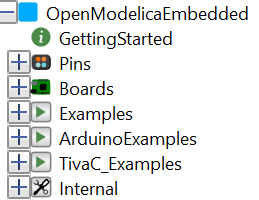
\includegraphics[width =0.5 \textwidth]{package_str}
\caption{Structure of OpenModelicaEmbedded package}
\label{figure:1}
\end{figure}

\section{SynchronizeRealTime Block}
This block is a part of Modelica\_DeviceDrivers library used for real-time simulation of the model, i.e., this block synchronizes simulation time of the process to real- time clock of the operating system. Without this block, the models designed using this package will not be able to give proper real-time output. This block works at five different priorty levels which can be changed in Parameters dialog box by double-clicking the block.

\begin{figure}[H]
\centering

\includegraphics[width = 0.3\textwidth]{realtime}
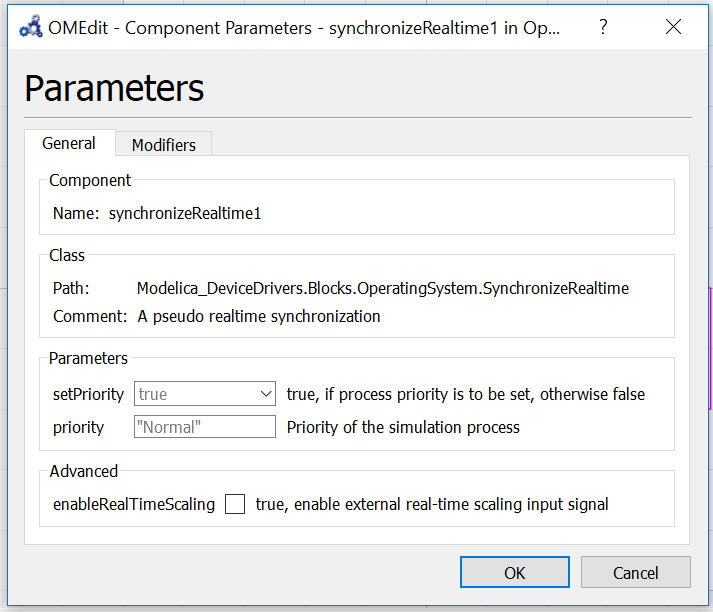
\includegraphics[width = 0.65\textwidth]{realtimepara}
\caption{SymchronizeRealTime block}
\label{figure:2}
\end{figure}

\section{Pins}
This package contains blocks which define to input and output pins of the board to which our hardware can be connected. These pin components define the properties and working of the pins used in the hardware.\\

\begin{itemize}
\item \textbf{AnalogInput:} It reads an analog signal from the specified pin. This component uses the function ‘analogRead’ of Arduino. It takes minimum and maximum values of the signal as parameter (default values being 0 and 1 respectively) and gives output depending on the size of ADC (analog to digital convertor) which is 10-bit for Arduino UNO board and 12-bit for Tiva C series TM4C123G board.
\begin{figure}[H]
\centering
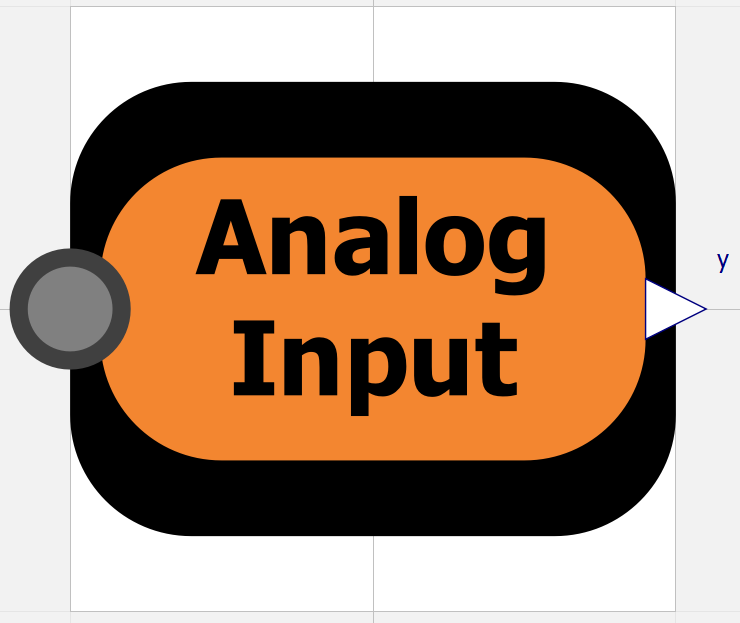
\includegraphics[width = 0.4\textwidth]{pin11}
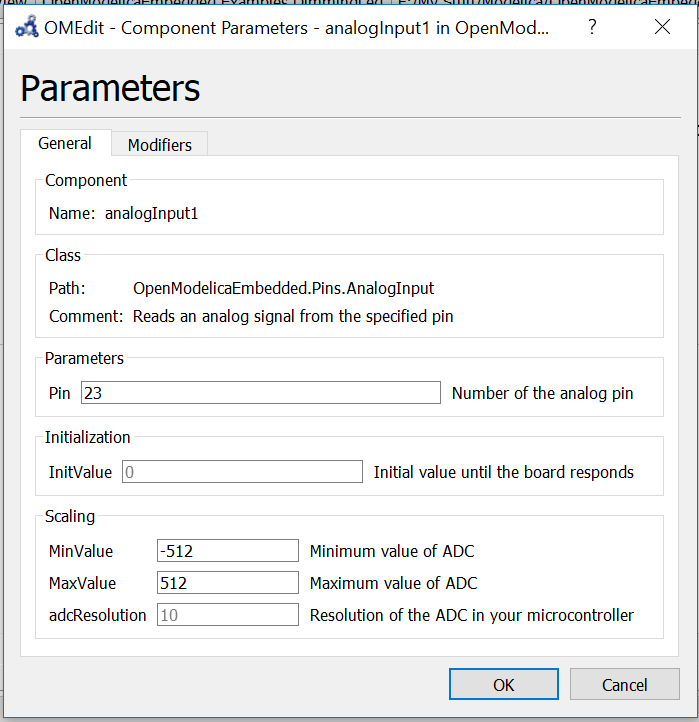
\includegraphics[width = 0.55\textwidth]{pin12}
\caption{AnalogInput block}
\label{figure:3}
\end{figure}
\item \textbf{AnalogOutput:} It writes analog value (PWM wave) to the specified pin. This component uses the function ‘analogWrite’ of Arduino. It takes minimum and maximum values of the signal as parameter (default values being 0 and 1 respectively) and gives output depending on the size of ADC.
\begin{figure}[H]
\centering
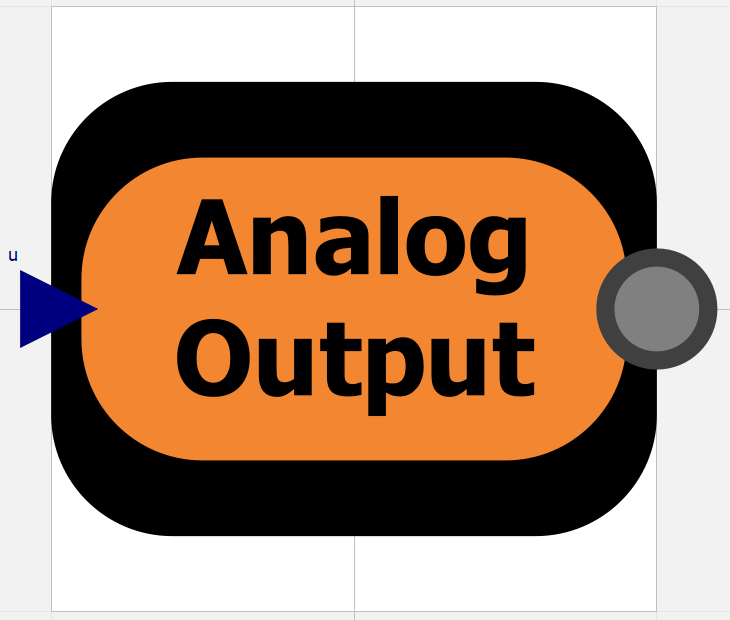
\includegraphics[width = 0.4\textwidth]{pin21}
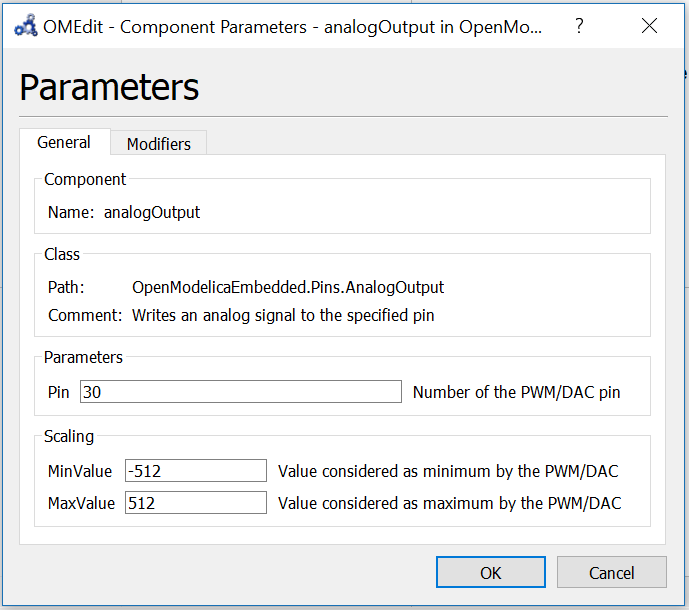
\includegraphics[width = 0.55\textwidth]{pin22}
\caption{AnalogOutput block}
\label{figure:4}
\end{figure}
\item \textbf{DigitalInput:} It reads an digital signal from the specified pin. This component uses the function ‘digitalRead’ of Arduino. It only takes boolean signals.
\begin{figure}[H]
\centering
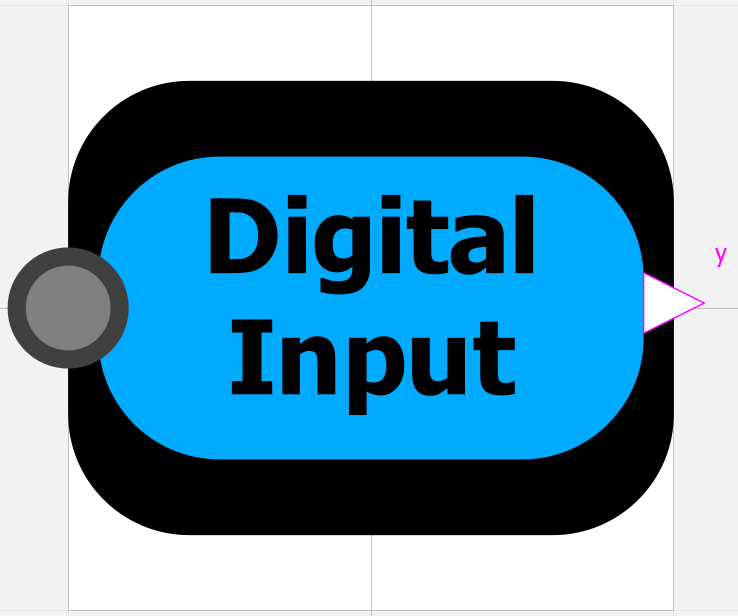
\includegraphics[width = 0.4\textwidth]{pin31}
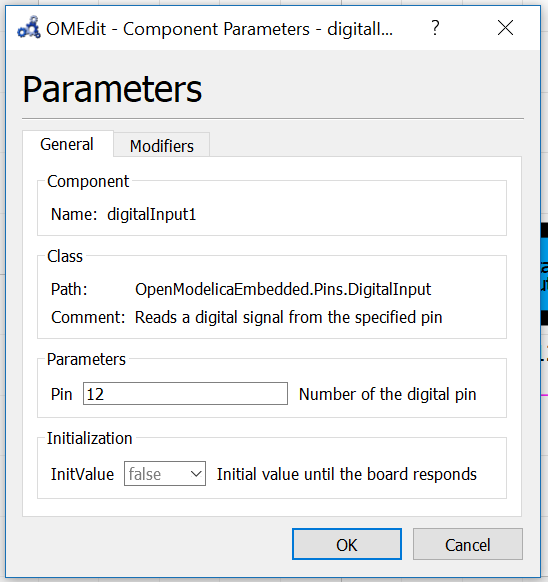
\includegraphics[width = 0.55\textwidth]{pin32}
\caption{DigitalInput block}
\label{figure:5}
\end{figure}
\item \textbf{DigitalOutput:} It writes digital value to the specified pin. This component uses the function ‘digitalWrite’ of Arduino. It only takes boolean signals.
\begin{figure}[H]
\centering
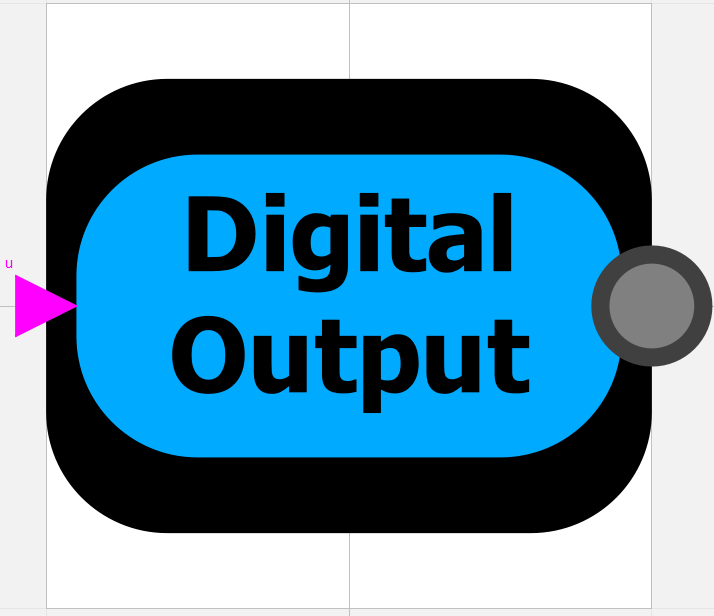
\includegraphics[width = 0.4\textwidth]{pin41}
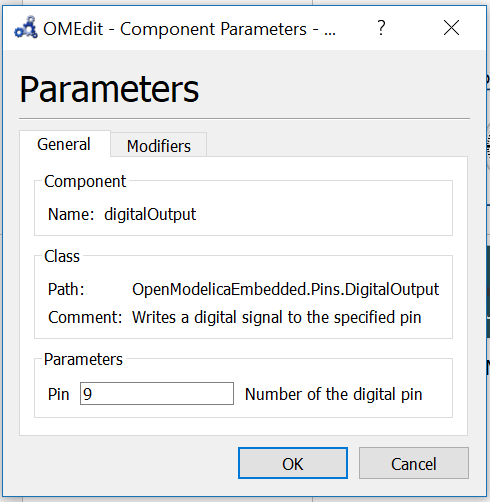
\includegraphics[width = 0.55\textwidth]{pin42}
\caption{DigitalOutput block}
\label{figure:6}
\end{figure}
\item \textbf{Servo:} It controls a servo motor attached to the specified pin. This component uses the 'Servo' library of Arduino. By default, the range goes from 0 to 1, which corresponds to 0 to 180 degrees. If you want to input values in degrees or radians, you can change the parameter 'InputUnit' to 'Degrees' or 'Radians'.
\begin{figure}[H]
\centering
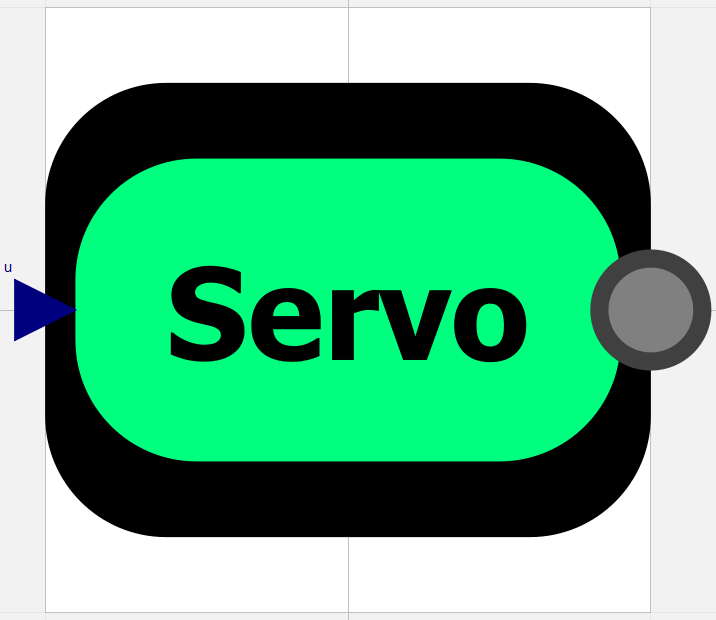
\includegraphics[width = 0.4\textwidth]{pin51}
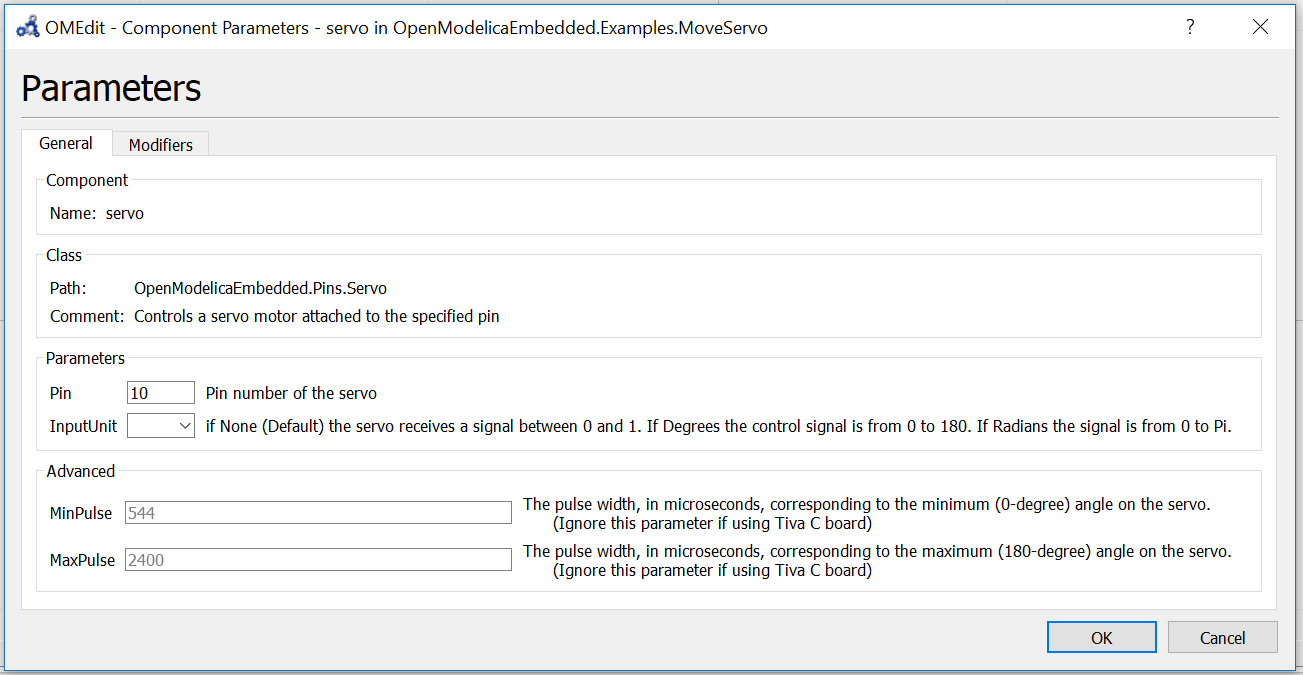
\includegraphics[width = 0.55\textwidth]{pin52}
\caption{Servo block}
\label{figure:7}
\end{figure}
\end{itemize}

\section{Boards}
This package contains block components which enable connection with different firmata boards. These components take serial port used for connection as parameter.		
\begin{itemize}
\item \textbf{Arduino:} Used for connecting to Arduino boards, such as Arduino UNO, Arduino Mega 2500 and others having similar firmata.
\begin{figure}[H]
\centering
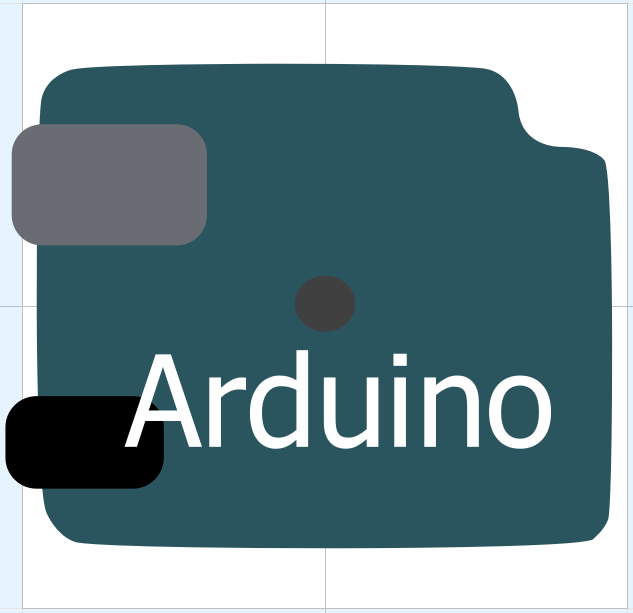
\includegraphics[width =0.25 \textwidth]{board1}
\caption{Arduino block}
\label{figure:8}
\end{figure}
\item \textbf{ArduinoLeonardo:} Supports Arduino Leonardo board and other boards using native USB.
\begin{figure}[H]
\centering
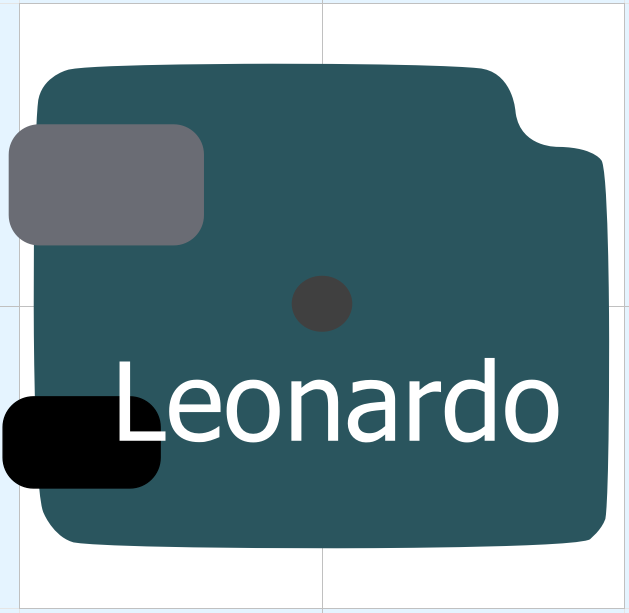
\includegraphics[width =0.25 \textwidth]{board2}
\caption{ArduinoLeonardo block}
\label{figure:9}
\end{figure}
\item \textbf{StandardFirmata:} Connects to Arduino compatible boards.
\begin{figure}[H]
\centering
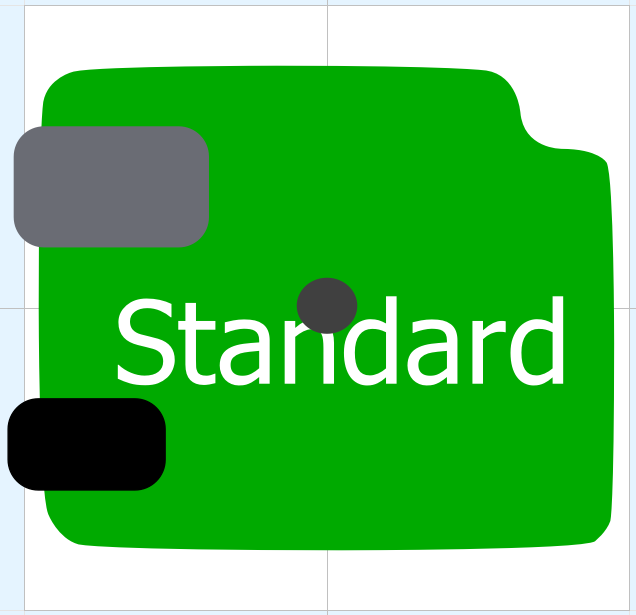
\includegraphics[width =0.25 \textwidth]{board3}
\caption{StandardFirmata block}
\label{figure:10}
\end{figure}
\item \textbf{CustomFirmata:} Supports any board firmata.
\begin{figure}[H]
\centering

\includegraphics[width =0.25 \textwidth]{board4}
\caption{CustomFirmata block}
\label{figure:11}
\end{figure}
\item \textbf{customBoard:} Takes name of the board also as parameter and can be used to connect any board supporting firmata.
\begin{figure}[H]
\centering
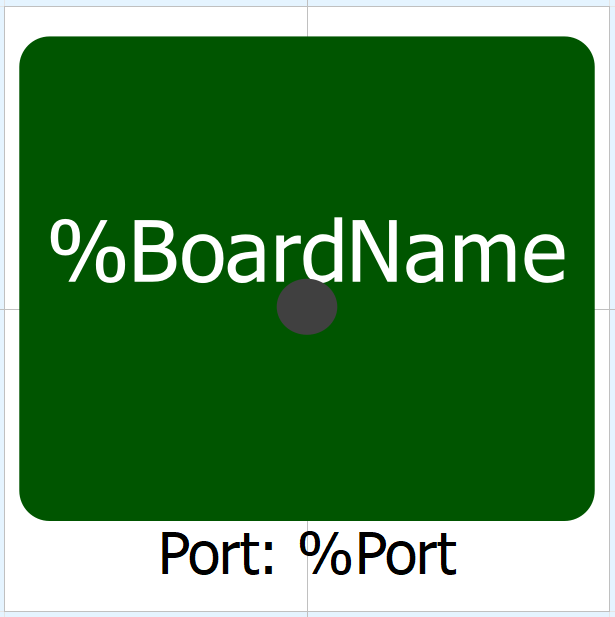
\includegraphics[width =0.25 \textwidth]{board5}
\caption{customBoard block}
\label{figure:12}
\end{figure}
\end{itemize}

\section{Examples}
The package contains example models to get introduced to the working of components of the package. These models accomplish different tasks using different blocks provided in Pins and Boards package. 

\section{ArduinoExamples}
The package contains example models specifc to Arduino UNO board. It can be used for other Arduino boards by change Pin Number parameter for the Pin blocks. Detailed description for the package is given in 'Working with Arduino'.

\section{TivaC\_Examples}
The package contains example models specifc to Tiva C Launchpad TM4C123G board. It can be used for other similar boards by change Pin Number parameter for the Pin blocks. Detailed description for the package is given in 'Working with Tiva C'. 

\section{Internal}
The components of this package cannot be used directly in the models. This package consists of icons and connectors defined and used for block designing, new types defined and used for the blocks and functions designed using external C/C++ functions at backend.

\chapter{\textbf{Hardware In Loop Simulation}}
\tab Hardware-in-the-loop (HIL) simulation, or HWIL, is a technique that is used in the development and test of complex real-time embedded systems. HIL simulation provides an effective platform by adding the complexity of the plant under control to the test platform. The complexity of the plant under control is included in test and development by adding a mathematical representation of all related dynamic systems. These mathematical representations are referred to as the “plant simulation”. The embedded system to be tested interacts with this plant simulation.\\

A HIL simulation must include electrical emulation of sensors and actuators. These electrical emulations act as the interface between the plant simulation and the embedded system under test. The value of each electrically emulated sensor is controlled by the plant simulation and is read by the embedded system under test (feedback). Likewise, the embedded system under test implements its control algorithms by outputting actuator control signals. Changes in the control signals result in changes to variable values in the plant simulation.

\section{Implementation}
\tab The package developed (OpenModelicaEmbedded) has several components like micro-controller boards, Digital/Analog Pins, etc. which you will have to use in your model to make it interact with connected hardware device. These components make calls to external C functions present in the library provided in Library directory. Those functions using serial communication communicate with the connected device. This source file will remain same irrespective of the connected hardware device and platform used (Windows, Linux, Mac).\\

The connected hardware device uses Firmata protocol to communicate with OpenModelica. The source code implementing Firmata protocol on hardware will vary depending on the language/ IDE used by that hardware/microcontroller, but the underlying protocol remains the same.

\chapter{\textbf{PID Controller}}
A \textbf{proportional - integral - derivative controller} (\textbf{PID controller} or \textbf{three term controller}) is a control loop feedback mechanism widely used in industrial control systems and a variety of other applications requiring continuously modulated control. A PID controller continuously calculates an error value e(t) as the difference between a desired setpoint (SP) and a measured process variable (PV) and applies a correction based on proportional, integral, and derivative terms (denoted P, I, and D respectively) which give the controller its name.

\section{Implementation}
The PID is implemented in the Firmware present on the hardware device using ‘AutoPID’ Library. To use the hardware for PID you will have to change the Firmware (Arduino source code) a bit by following the instructions mentioned in the Firmware itself. The only thing you have to do is just comment/uncomment a few macros depending on your application.

\begin{figure}[H]
\centering
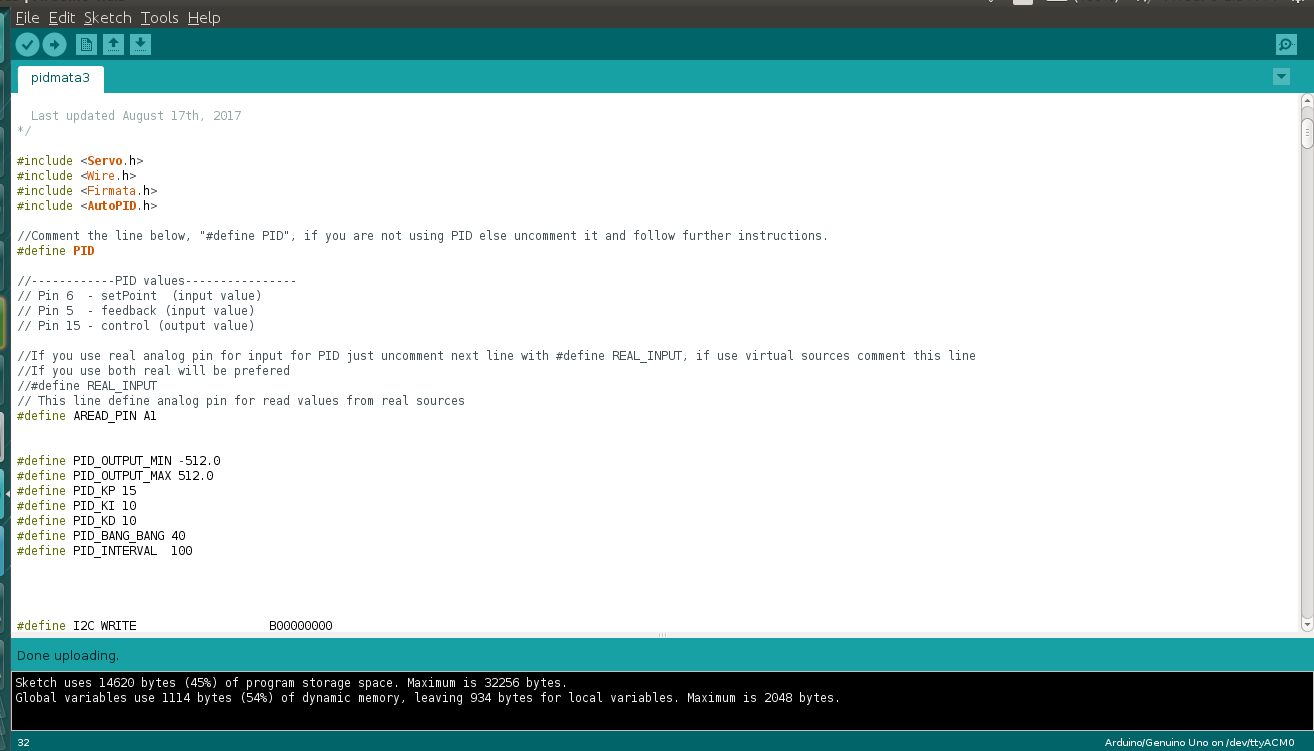
\includegraphics[width =0.9\textwidth]{pid}
\caption{Firmata to work with PID Controller}
\label{figure:24}
\end{figure}

\section{Example for PID}
\textbf{Example:} DCMotorWithPID (from Examples package)
\begin{figure}[H]
\centering
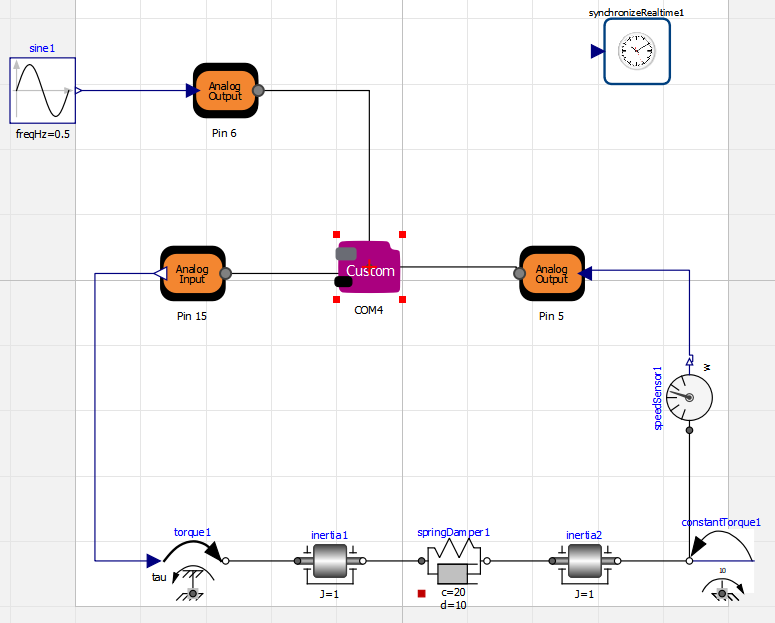
\includegraphics[width =0.9\textwidth]{pid_ex}
\caption{Model for PID Controller with DC Motor}
\label{figure:25}
\end{figure}
\begin{figure}[H]
\centering
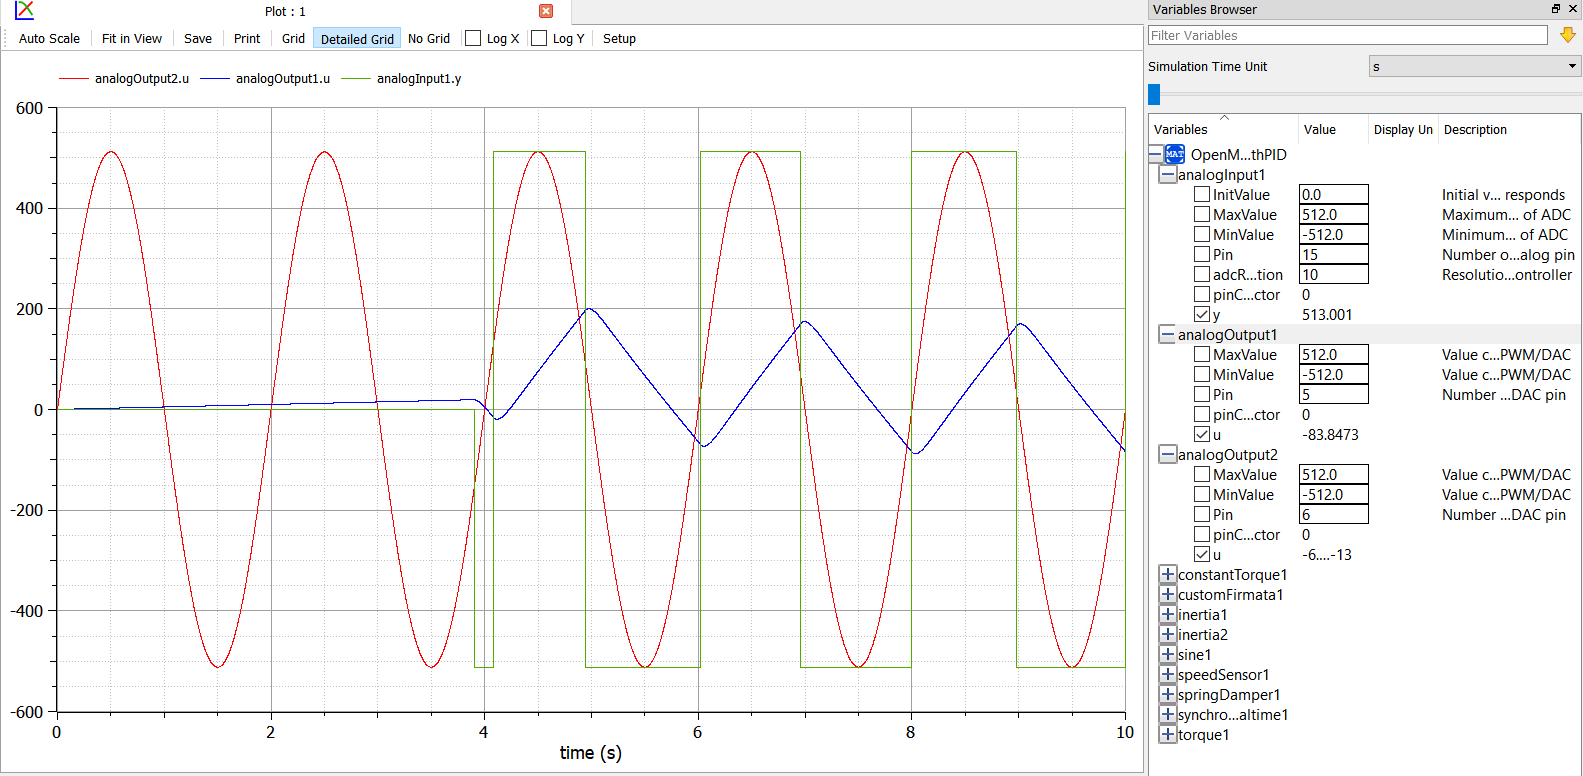
\includegraphics[width = 0.9\textwidth]{pid_graph}
\caption{Plot for PID Controller with DC Motor}
\label{figure:26}
\end{figure}

\chapter{\textbf{Working with Arduino UNO}}
The Arduino UNO is a widely used microcontroller board based of ATmega328P microcontroller IC and is developed by Arduino.cc. It operates at a voltage of 5V. The board contains 14 Digital and 6 Analog input/output (I/O) pins, a 10-bit ADC (Analog to Digital Convertor), 8-bit DAC, a in-built LED connected to digital pin no. 13 and many other features.

\begin{figure}[H]
\centering
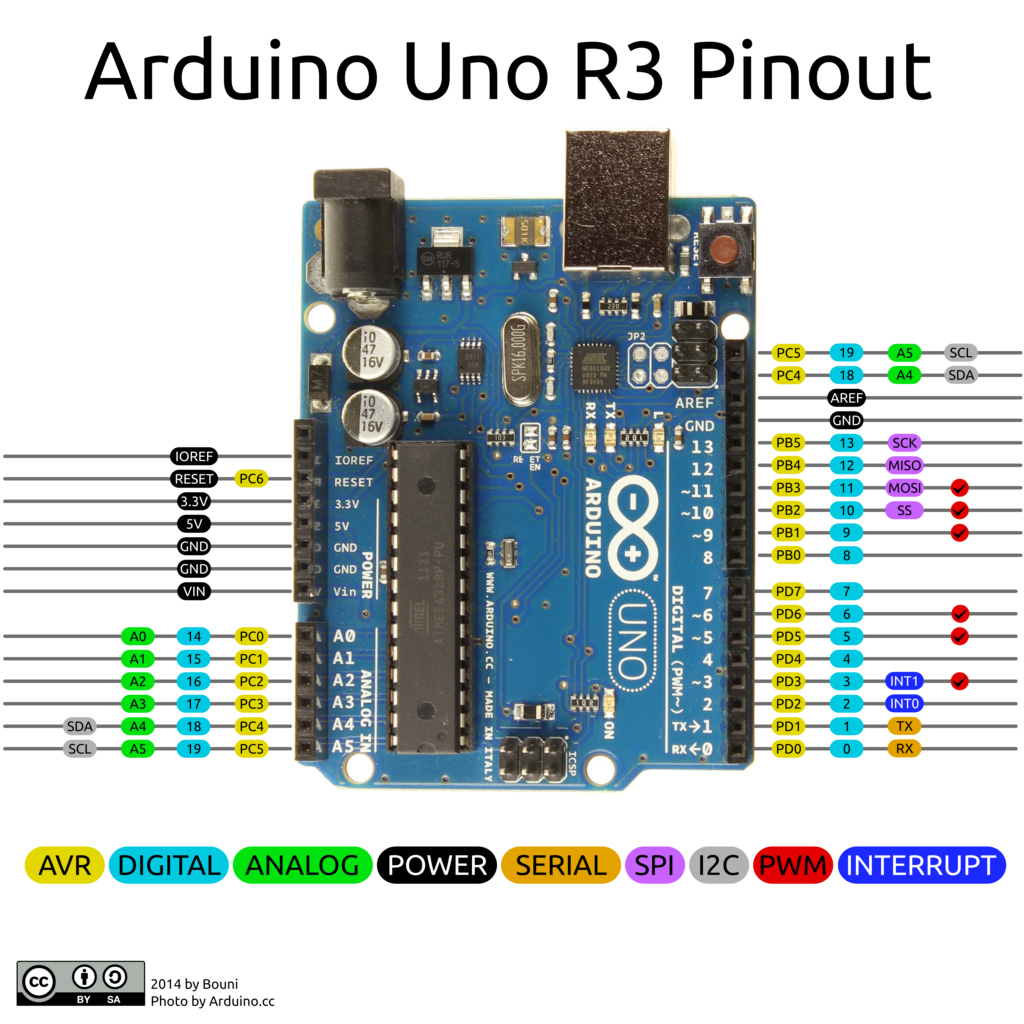
\includegraphics[width =0.75 \textwidth]{arduino_uno_pinout}
\caption{Pin Diagram of Arduino UNO}
\label{figure:13}
\end{figure}

\section{Connecting and Configuring the Board}
\begin{enumerate}
\item Connect the Arduino UNO board to the computer using a USB cable.
\item Open Arduino IDE.
\item In Tools Menu, select Board \textrightarrow Arduino/Genuino UNO  and Port as the available serial port to which Arduino is connected.
\item The serial port can be identified by:\\
For Linux:\\
Type the command \textbf{ls -l /dev/ttyACM*} in the terminal and the output it returns gives the port to which Arduino is connected, for example \textbf{/dev/ttyACM0}.\\
For Windows:\\
Open \textbf{Device Manager} and check for the name of connected port which will be in the form, for example, \textbf{COM5}.
\item Click Sketch \textrightarrow Include libraries and select Manage libraries, type AutoPID in the search bar and install the library.
\item Click File \textrightarrow Open and browse OpenModelicaEmbedded \textrightarrow Firmware \textrightarrow Arduino \textrightarrow pidmata3 and open pidmata3.ino.\\
OR\\
Open StandardFirmata sketch: File \textrightarrow Examples \textrightarrow StandardFirmata , if not working with PID.\\
\item Upload the sketch to the board.
\end{enumerate}

\section{Interfacing with OpenModelica}
\begin{enumerate}
\item Upload StandardFirmata sketch to the Arduino board.
\item Open package.mo from OpenModelicaEmbedded package, also open package.mo file from Modelica\_DeviceDrivers library.
\item In OpenModelicaEmbedded package, open ArduinoExamples package.
\item In Diagram view, change the port name for the board component to the port to which board is connected by double-clicking on it.
\item Simulate the example model.	
\end{enumerate}

\section{Examples for Arduino}
ArduinoExamples package consists of example models designed for specificly to work with Arduino UNO board. In order to work with these examples, double-click of board block in the Diagram view and change port name to the port to which board is connected. If working with any other similar Arduino board, double-click the pin blocks and change pin number as per the used board.

\subsection{LED Examples}
\textbf{Example:} arduino\_ex1\_led\_blue\\

The following is an example to turn on the blue led indefinitely. Double clicking each block opens the parameter window for it. Change the parameters according to the following image.

\begin{figure}[H]
\begin{subfigure}{.5\textwidth}
\centering
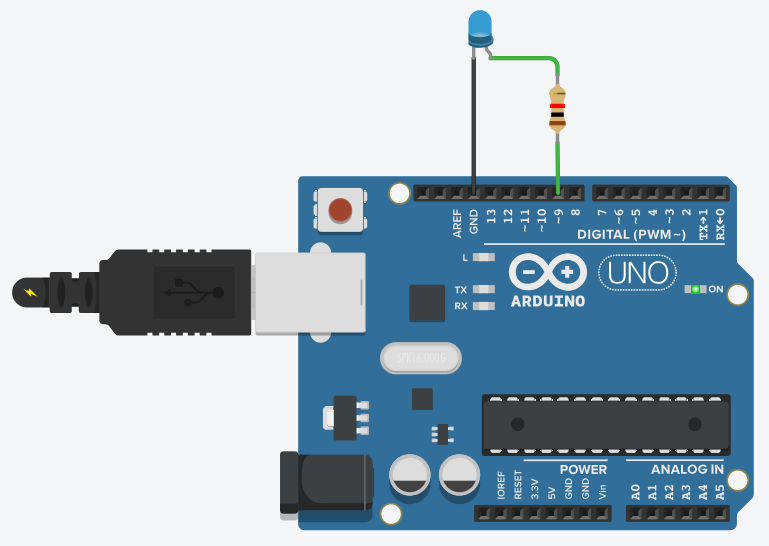
\includegraphics[width =\linewidth]{1}
\caption{Connections for lighting up blue led}
\end{subfigure}
\begin{subfigure}{.5\textwidth}
\centering
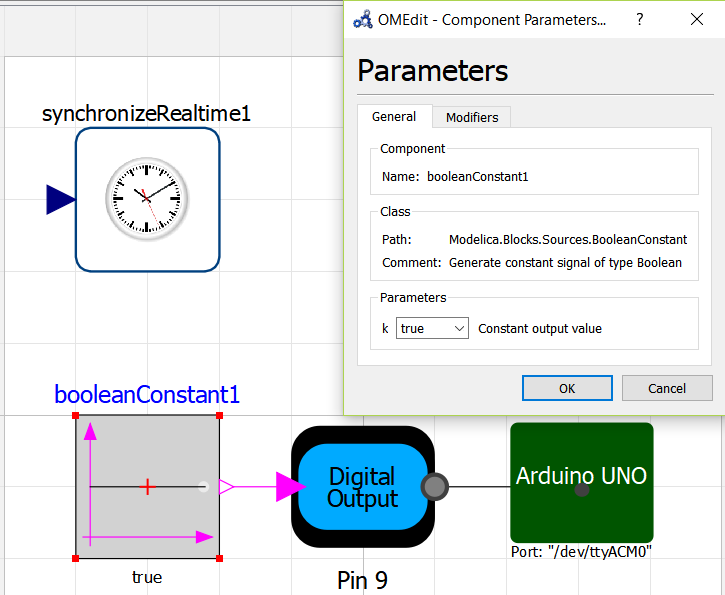
\includegraphics[width =\linewidth]{led_ex1}
\caption{Model for lighting up blue led}
\end{subfigure}
\caption {Arduino Led Example}
\label{figure:14}
\end{figure}

\subsection{Push Button Examples}
\textbf{Example:} arduino\_ex1\_push\_button\_status\\

The following example is to read the status of the pushbutton and display it on the serial monitor.\\

In this model, a BooleanValue block is used to show boolean value coming from the digital input pin of arduino on Simulation Output. The block BooleanValue can be found at Modelica.Blocks.Interaction.Show.BooleanValue.\\

Moreover, a print statement to print boolean value is written in the Text view of the model which can be seen in ~\ref{figure:23}.\\

Double clicking each block opens the parameter window for it. Change the parameters according to the following image.

\begin{figure}[H]
\begin{subfigure}{.5\textwidth}
\centering
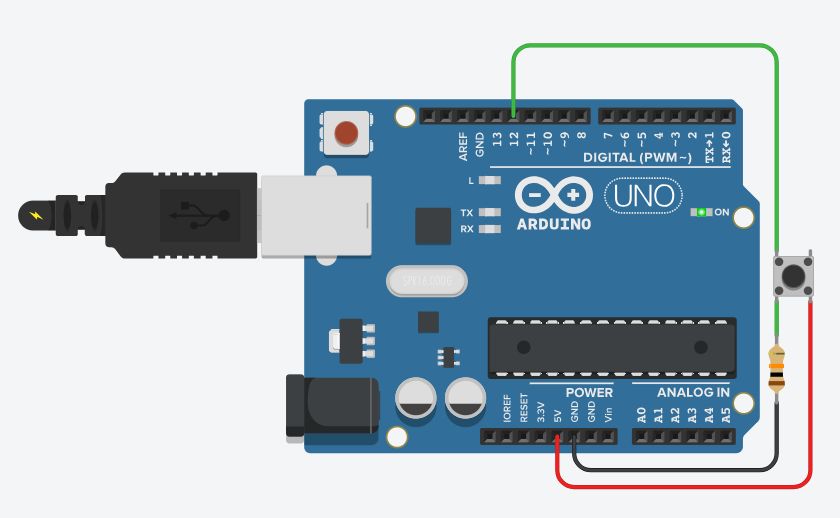
\includegraphics[width =\linewidth]{2}
\caption{Connections for push button}
\end{subfigure}
\begin{subfigure}{.5\textwidth}
\centering
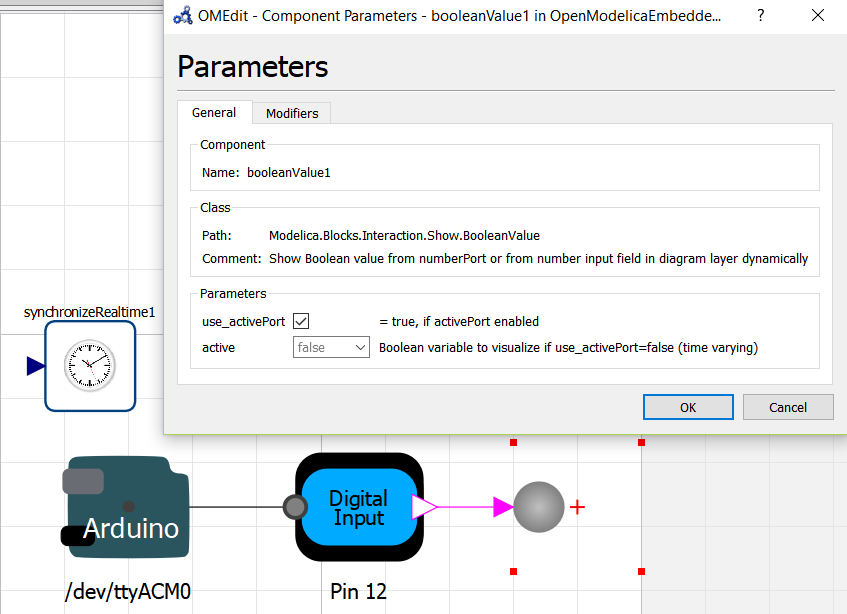
\includegraphics[width =\linewidth]{pb_ex1}
\caption{Model for checking status of push button}
\end{subfigure}
\caption {Arduino Push Button Example}
\label{figure:15}
\end{figure}

\begin{figure}[H]
\centering
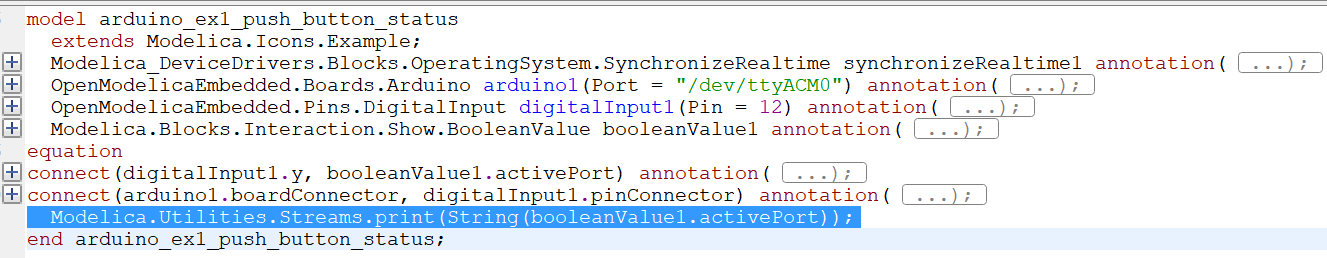
\includegraphics[width =\textwidth]{pb_ex1_print}
\caption{Print Statement}
\label{figure:23}
\end{figure}


\subsection{LDR Examples}
\textbf{Example:} arduino\_ex2\_ldr\_read\\

Turning the blue LED on and off according to the values of LDR (Light Dependent Resistor).\\

In this model, 2 blocks have been used namely Less and Constant.\\

Less block takes 2 input and gives 1 output according to the values of input. For example in the case below, when value from pin 19 is less than k = 300, output is true (or 1) and when value from pin 19 is greater than equal to k=300, its output is false (or 0). The block can be found at Modelica.Blocks.Logical.Less.\\

Constant block provides with a constant value which can be set by user. The block can be found at Modelica.Blocks.Sources.Constant.

\begin{figure}[H]
\begin{subfigure}{.5\textwidth}
\centering
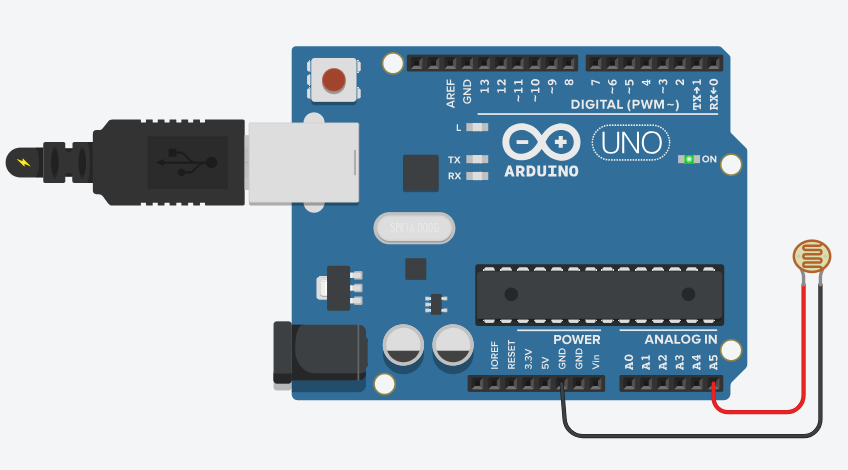
\includegraphics[width =\linewidth]{3}
\caption{Connections for ldr}
\end{subfigure}
\begin{subfigure}{.5\textwidth}
\centering
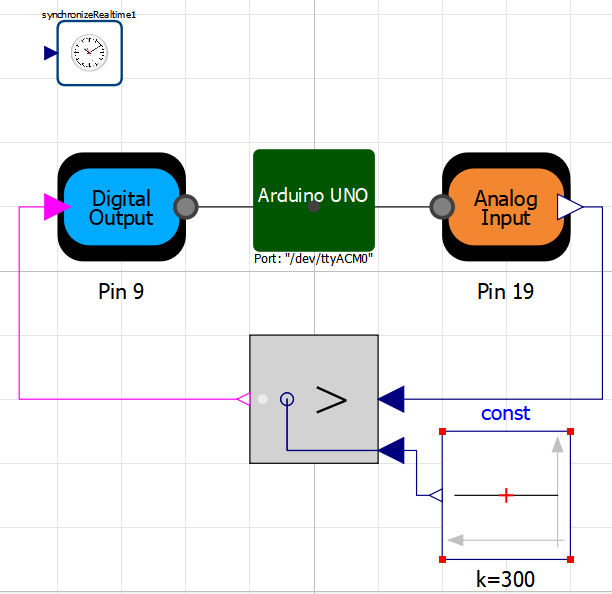
\includegraphics[width =\linewidth]{ldr_ex2}
\caption{Model for switching led depending on ldr value}
\end{subfigure}
\caption {Arduino LDR Example}
\label{figure:16}
\end{figure}

\subsection{DC Motor Examples}
\textbf{Example:} arduino\_ex2\_dcmotor\_both\\

The following example is of rotating the DC motor in both directions. As visible in the model below, 2 pulse blocks are used to manage this. \\

A pulse block generates pulse signals of real value. It’s amplitude, duty cycle, time period, start time can be varied through changing amplitude, width, period, startTime respectively in the parameter window of the pulse. The block can be found at Modelica.Blocks.Sources.Pulse.\\

Double clicking each block opens the parameter window for it. Change the parameters according to the following image.

\begin{figure}[H]
\begin{subfigure}{.75\textwidth}
\centering
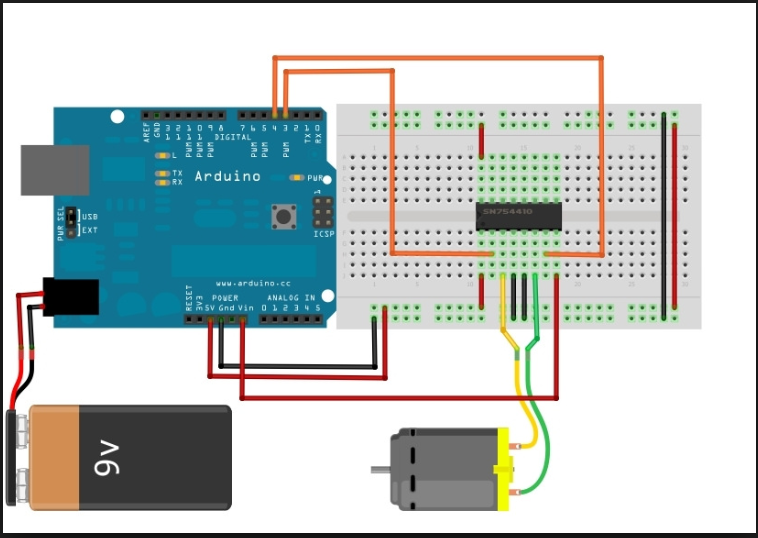
\includegraphics[width =\linewidth]{4}
\caption{Connections for dc motor}
\end{subfigure}
\begin{subfigure}{\textwidth}
\centering
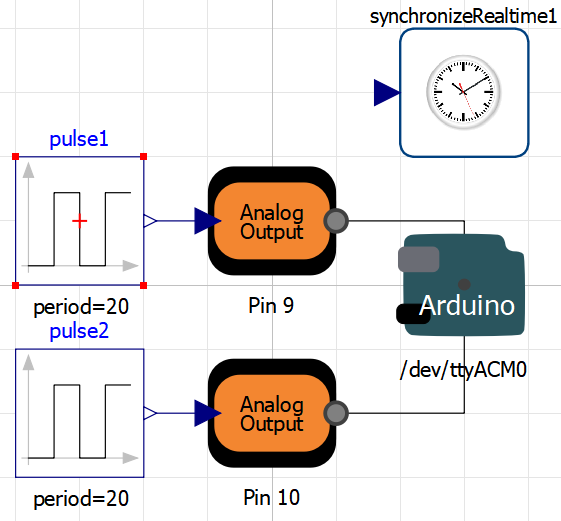
\includegraphics[width =0.3\linewidth]{dc_ex2}
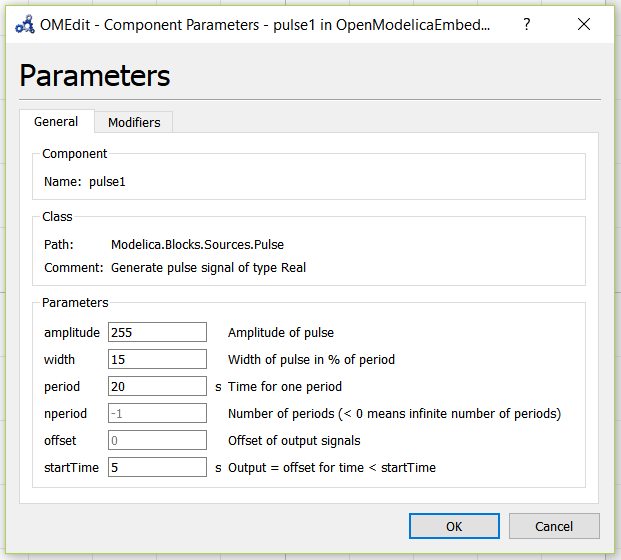
\includegraphics[width =0.3\linewidth]{dc_ex2_2}
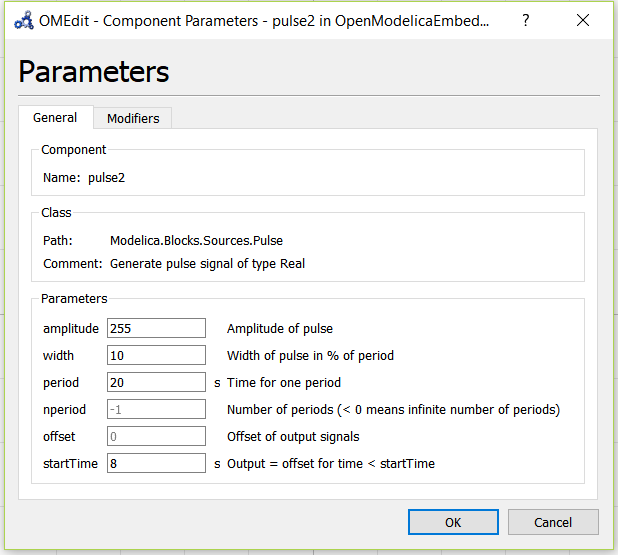
\includegraphics[width =0.3\linewidth]{dc_ex2_3}
\caption{Model for rotating dc motor in both directions}
\end{subfigure}
\caption {Arduino DC Motor Example}
\label{figure:17}
\end{figure}

\subsection{Potentiometer Examples}
\textbf{Example:} arduino\_ex1\_pot\_threshold\\

The following example is of turning on LEDs depending on the potentiometer threshold. As seen in the model below, we’ve used Xor and GreaterEqualThreshold blocks. \\

The GreaterEqualThreshold block has a parameter-threshold; if the input value to the block is greater than or equal to this threshold then the output is the same as input, otherwise 0.\\

This block can be found at Modelica.Blocks.Logical.GreaterEqualThreshold.\\

The other one is Xor block which simply xor’s ihe 2 input values it gets. This block can be found at Modelica.Blocks.Logical.Xor.

\begin{figure}[H]
\begin{subfigure}{.5\textwidth}
\centering
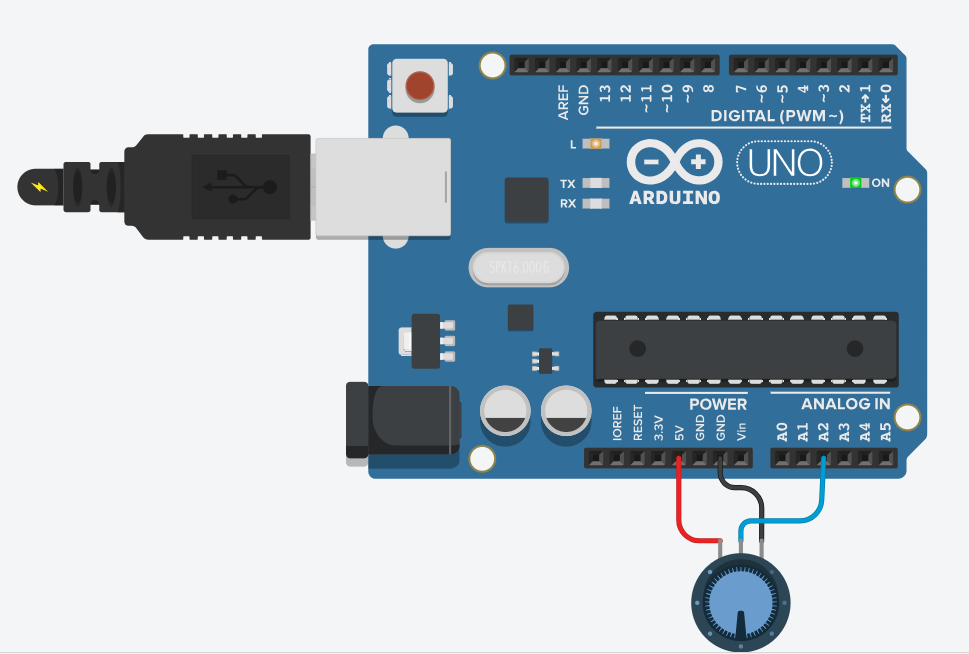
\includegraphics[width =\linewidth]{5}
\caption{Connections for potentiometer}
\end{subfigure}
\begin{subfigure}{.5\textwidth}
\centering
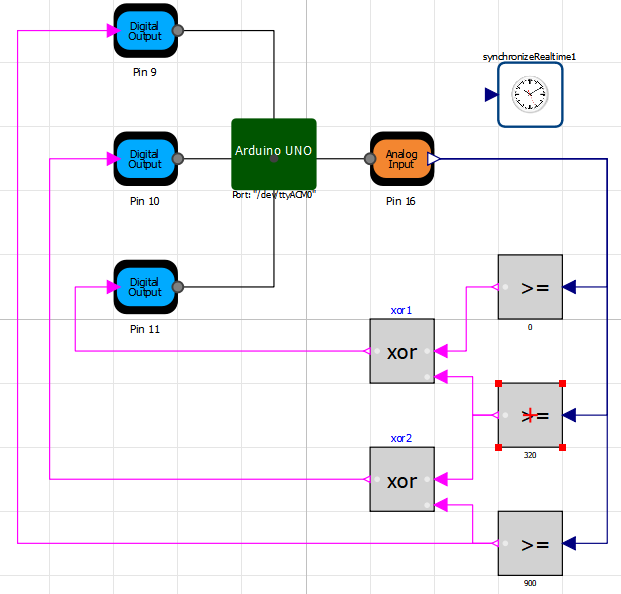
\includegraphics[width =\linewidth]{potentio_ex1}
\caption{Model for potentiometer threshold ranges}
\end{subfigure}
\caption {Arduino Potentiometer Example}
\label{figure:18}
\end{figure}

\subsection{Thermistor Examples}
\textbf{Example:} arduino\_ex1\_therm\_read\\

Turning the buzzer on and off using the thermistor values read by ADC. \\

It’s model has Greater block. Greater block takes 2 input and gives 1 output according to the values of input. For example in the case below, when value from pin 18 is greater than k = 500, output is true(or 1) and when value from pin 18 is less than equal to k=500, its output is false(or 0). The block can be found at Modelica.Blocks.Logical.Greater.

\begin{figure}[H]
\begin{subfigure}{.5\textwidth}
\centering
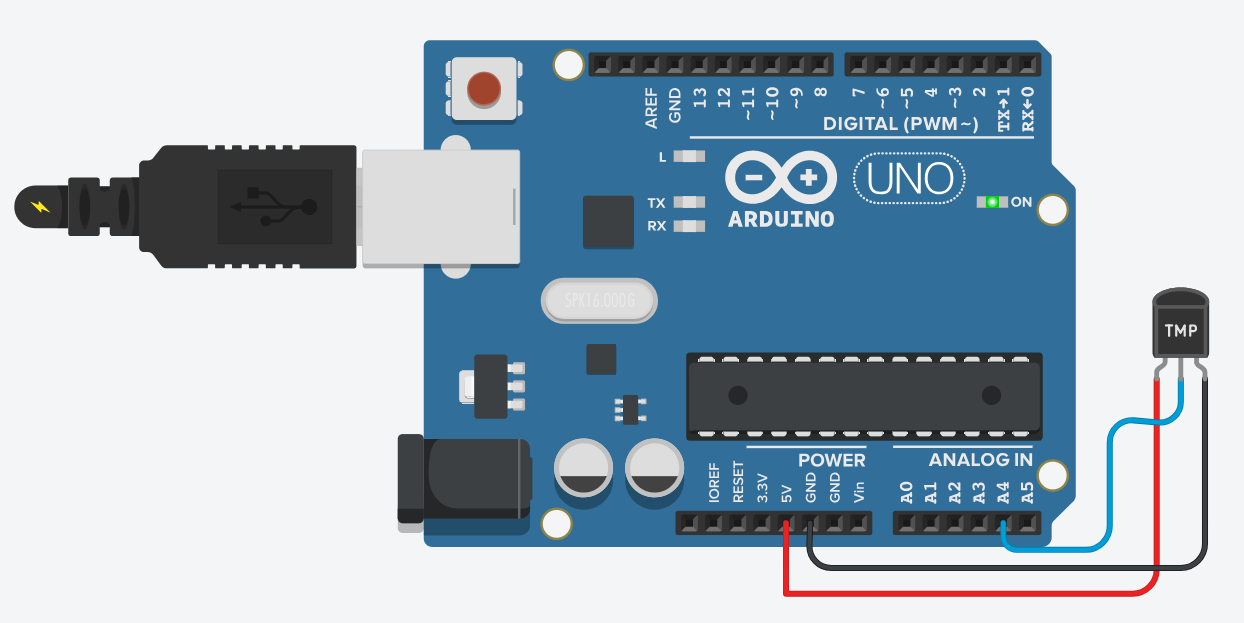
\includegraphics[width =\linewidth]{6}
\caption{Connections for thermistor}
\end{subfigure}
\begin{subfigure}{.5\textwidth}
\centering
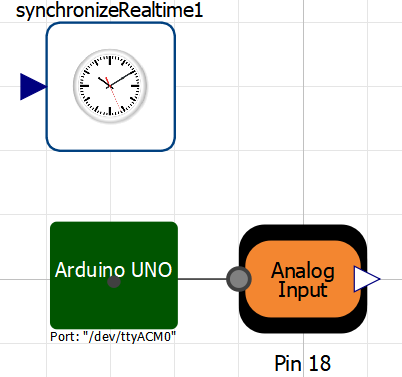
\includegraphics[width =\linewidth]{thermistor_ex1}
\caption{Model for checking value of thermistor}
\end{subfigure}
\caption {Arduino Thermistor Example}
\label{figure:19}
\end{figure}

\subsection{Servo Motor Examples}
\textbf{Example:} arduino\_ex3\_servo\_loop\\

Rotating the servo in increments. \\

The model contains blocks like Product, RealToInteger, IntegerToReal, Constant and Ramp. The Ramp block gives a strictly increasing value. On using RealToInteger block on the output, it converts it to step function. Now as the Product block accepts 2 input in real format only, there was a need to convert the value back to real using IntegerToReal block.\\

In Servo pin, set InputUnit to OpenModelicaEmbedded.Internal.Types.ServoUnit.None. \\

As can be seen from data sheet (Figure:~\ref{figure:27}) SG90 has a duty cycle of 5-10\% where if it is 5\%, the position of motor is -90 degrees and if 10\%, it is +90 degrees. So as we were simulating for 10 seconds, MinPulse was 0.5 sec and MaxPulse was 1sec in Servo pin Parameters.

\begin{figure}[H]
\centering
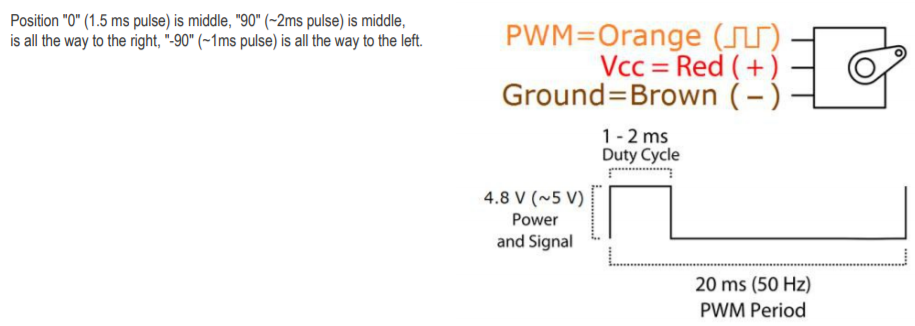
\includegraphics[width =\textwidth]{servo_datasheet}
\caption{Data Sheet for Servo Motor SG90}
\label{figure:27}
\end{figure}

\begin{figure}[H]
\begin{subfigure}{.5\textwidth}
\centering
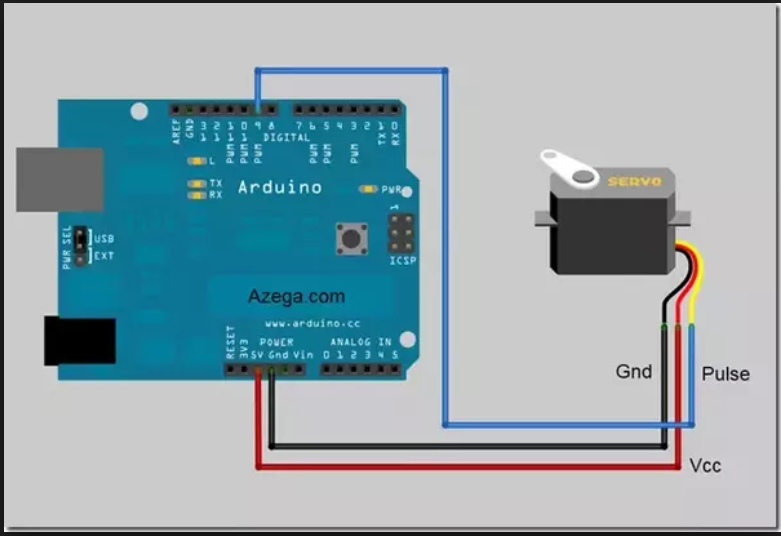
\includegraphics[width =\linewidth]{7}
\caption{Connections for Servo Motor}
\end{subfigure}
\begin{subfigure}{.5\textwidth}
\centering
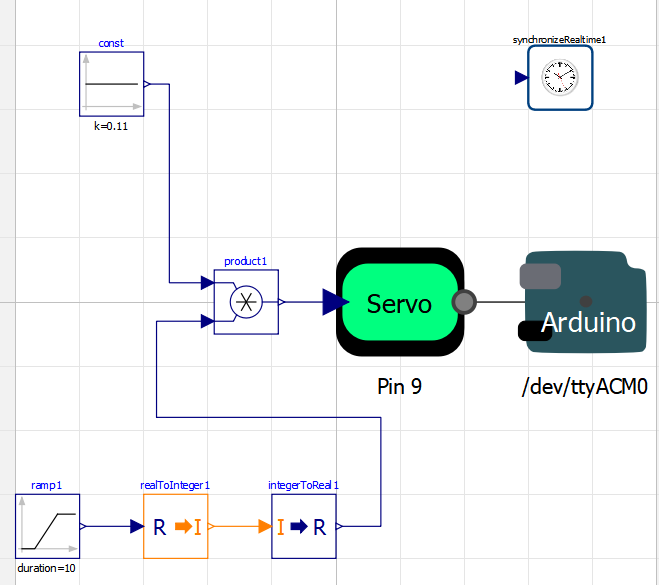
\includegraphics[width =\linewidth]{servo_ex3}
\caption{Model for working with Servo Motor}
\end{subfigure}
\caption {Arduino Servo Motor Example}
\label{figure:20}
\end{figure}

\chapter{\textbf{Working with Tiva C Launchpad}}
The Tiva C series Launchpad Evaluation board (EK-TM4C123GXL) is low cost ARM-Cortex-M4F based microcontroller.	 The board contains 40 I/O pins, two user programmable push buttons, a RGB led and many more features.

\begin{figure}[H]
\centering
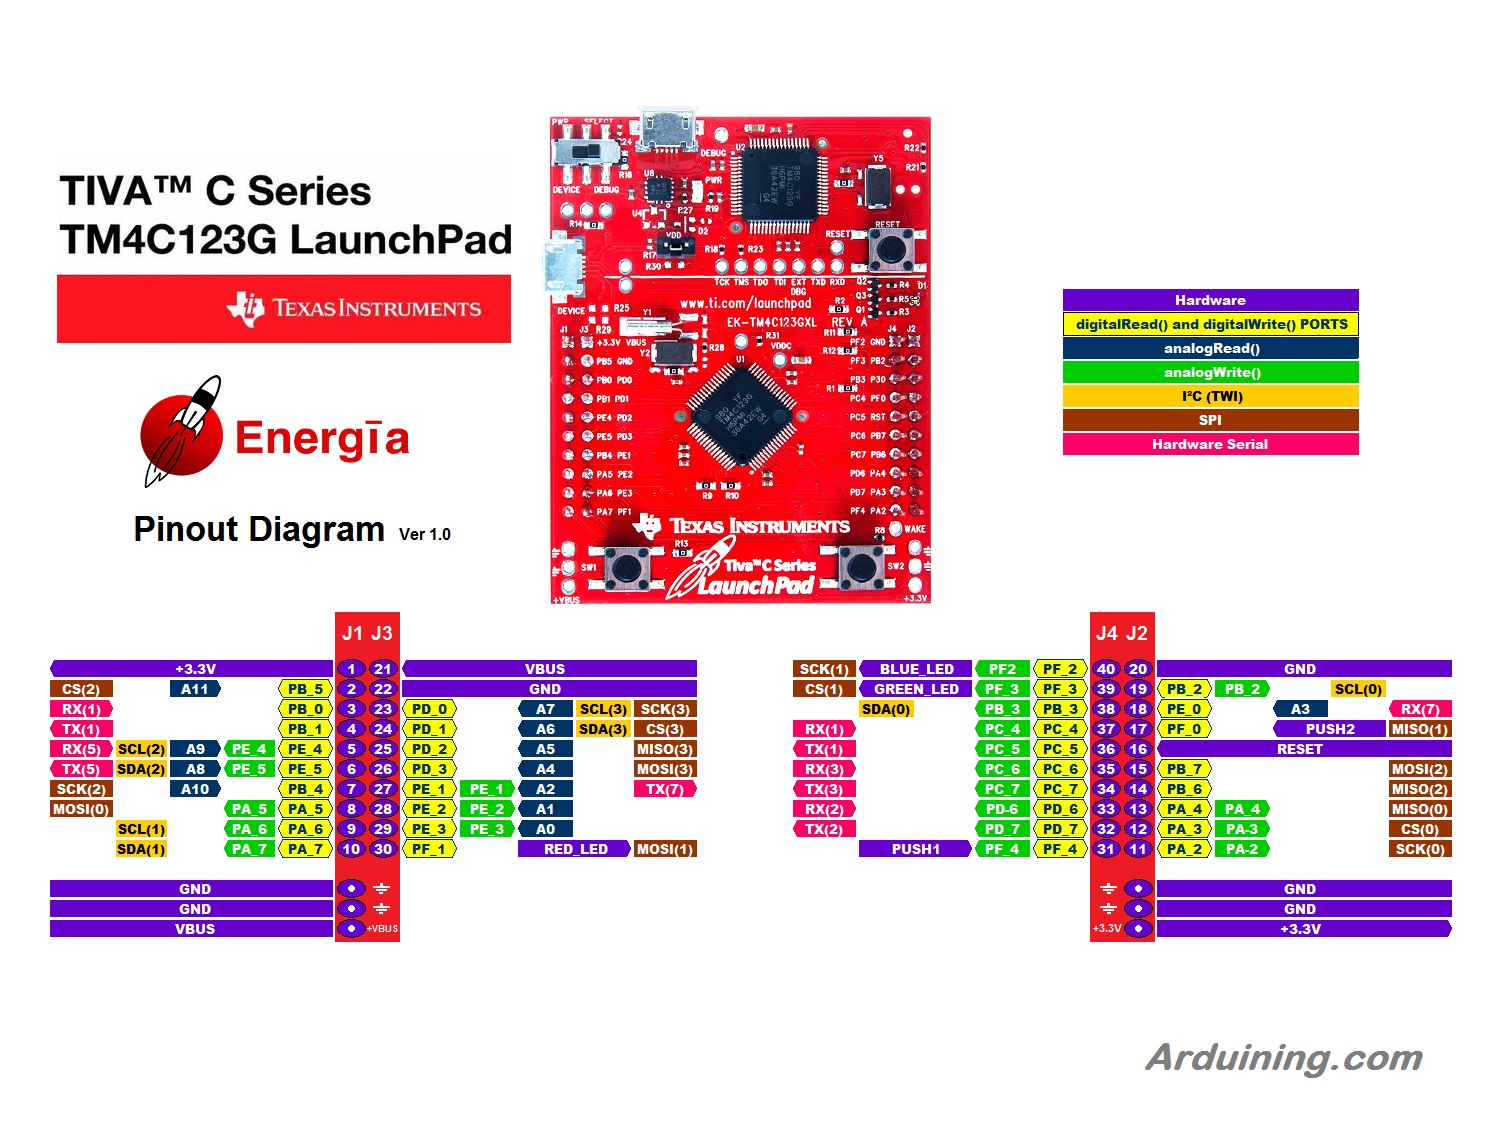
\includegraphics[width =\textwidth]{tiva_c_launchpad_pinout}
\caption{Pin Diagram of Tiva C Launchpad}
\label{figure:21}
\end{figure}

\section{Connecting and Configuring the Board}
\begin{enumerate}
\item Connect the Tiva C board to the computer using a USB cable.
\item Open Energia IDE.
\item In Tools Menu, select Board \textrightarrow Tiva C  and Port as the available serial port to which Arduino is connected.
\item If Tiva C board is not present, then click on Board Manager, type Tiva C in search bar and then click on Install to install board library, then apply Step 3.
\item In Sketch menu, Select Include Library \textrightarrow Add .zip library and add the zip file provided in the Firmware folder. Then open StandardFirmata sketch: File \textrightarrow Examples \textrightarrow StandardFirmata.\\
OR\\
Click File \textrightarrow Open and browse OpenModelicaEmbedded \textrightarrow Firmware \textrightarrow Tiva C \textrightarrow StandardFirmata and open StandardFiramata.ino.
\item Upload the sketch to the board.
\end{enumerate}

\section{Interfacing with OpenModelica}
\begin{enumerate}
\item Upload StandardFirmata sketch to the Tiva C board.
\item Open package.mo from OpenModelicaEmbedded package, also open package.mo file from Modelica\_DeviceDrivers library.
\item In OpenModelicaEmbedded library, open TivaC\_Examples package.
\item In Diagram view, change the port name for the board component to the port to which board is connected by double-clicking on it.
\item Simulate the example model.
\end{enumerate}

\section{Examples for Tiva C}
The examples explained in package for tiva-c are same as that for arduino board except that the pin configurations are different. The configuration can be seen from the pin diagram from Figure~\ref{figure:21}.\\

\textbf{Example:} tivac\_ex1\_led\_blue
\begin{figure}[H]
\centering
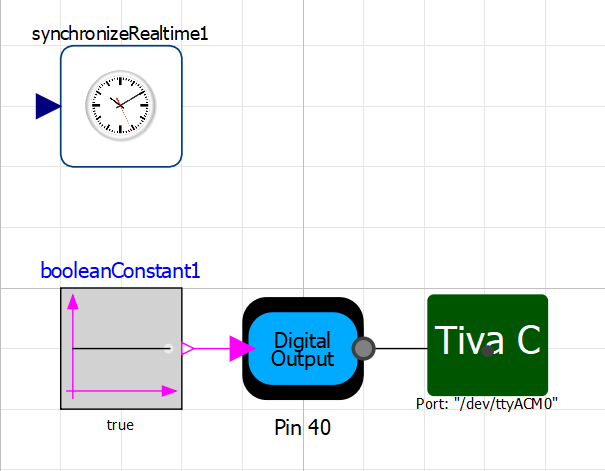
\includegraphics[width =0.75\textwidth]{tiva_led}
\caption{Tiva C Led Example}
\label{figure:22}
\end{figure}
The example Tiva-C Led works same as the one which is explained for arduino except for the fact that the pin configuration has been changed,for arduino it was pin number 9 while for tiva-c board it is pin number 40 as can be reffered from the pin diagram of tiva-c board (Figure: ~\ref{figure:21}). All other working remains same as already explained in case of Arduino.\\

For all other models also only pin number changes in case of Arduino rest they are similar to those present in ArduinoExamples package.

\chapter{\textbf{Conclusion}}
\tab The project "Interfacing of Embedded Systems with OpenModelica", is based on implementing an example package for Arduino board as well as for tiva-C board.We implemented the same set of examples on both Arduino board as well as Tiva-c board because Tiva-c board targets industries.We implemented hardware in loop simulation and PID tuning was done. Indeed the same set of codes can be used for linux as well as for windows plateform. We also explored the embedded targets package of the Modelica\_DeviceDrivers library.\\

Although, there were many issues initially, most of them got resolved in the course of the project. While working on the project with OpenModelica we came to a conclusion that OpenModelica is an open source software based on Modelica language to design and simulate complex physical systems through code as well as graphical blocks which is also very useful for electronics prototyping and real time simulations. The main drawback of the library is its lack of appropriate documentation and various other hardware supports in the electronics hardware area. Such modules are open for modifications and can be extended by future developers. Therefore we have explored OpenModelica in detail and tried to provide a better insight in this open source software which will help developers in the future.

\newpage
\title{\textbf{\textbf{\LARGE 
\begin{flushleft}
\textbf{Reference}
\end{flushleft}
}}}
The following sources were referred to while working on this project:
\begin{itemize}
\item  Peter Fritzson :Principles of Object-Oriented Modeling and Simulation with Modelica 3.3: A Cyber-Physical Approach
\item \url{ https://www.openmodelica.org/}
\item \url{ http://book.xogeny.com/}
\item \url{ https://build.openmodelica.org/Documentation/Modelica.html}
\item \url{ https://www.codeproject.com/Articles/84461/MinGW-Static-and-Dynamic-Libraries}
\item \url{https://stackoverflow.com/questions/10039401/use-32bit-shared-library-from-64bit-application}
\item \url{ https://stackoverflow.com/questions/142508/how-do-i-check-os-with-a-preprocessor-directive}
\item \url{https://en.wikipedia.org/wiki/PID_controller}
\item \url { https://openmodelica.org/doc/OpenModelicaUsersGuide/latest/interop_c_python.html}
\end{itemize}

\end{document}


